\documentclass{beamer}

% Theme
\usetheme{Madrid}
\usecolortheme{default}

% Packages
\usepackage{amsmath,amssymb,amsfonts}
\usepackage{graphicx}
\usepackage{xcolor}
\usepackage{tikz}
\usepackage{tkz-euclide}
\usepackage{array}
\usepackage{multirow}
\usepackage{longtable}
\usepackage{lscape}
\usepackage{listings}
\lstset{
    basicstyle=\ttfamily\small,
    keywordstyle=\color{blue},
    commentstyle=\color{gray},
    stringstyle=\color{red},
    showstringspaces=false,
    breaklines=true
}

% Custom macros
\newcommand{\myvec}[1]{\begin{pmatrix}#1\end{pmatrix}}
\newcommand{\brak}[1]{\left( #1 \right)}
\newcommand{\augvec}[3]{%
  \left(\!\begin{array}{@{}*{#1}{r}|*{#2}{r}@{}}#3\end{array}\!\right)
}

% Redefine \vec to bold letters only (no arrow)
\renewcommand{\vec}[1]{\mathbf{#1}}

\title{5.8.17}
\author{EE25BTECH11019 -- Darji Vivek M.}
\date{}

\begin{document}

\begin{frame}
\begin{titlepage}

\end{titlepage}
\end{frame}
\begin{frame}{Question}
\textbf{Question:}\\
A fraction becomes $\frac{9}{11}$ if $2$ is added to both the numerator and the denominator. If $3$ is added to both the numerator and the denominator, it becomes $\frac{5}{6}$. Find the fraction.\\[4pt]
\end{frame}

\begin{frame}{Solution}
\textbf{Matrix Method:}\\
Let the numerator be $n$ and the denominator be $d$.\\[4pt]
From the given conditions,
\begin{align}
\frac{n+2}{d+2} &= \frac{9}{11}
\implies 11(n+2)=9(d+2)
\implies 11n-9d=-4,\\
\frac{n+3}{d+3} &= \frac{5}{6}
\implies 6(n+3)=5(d+3)
\implies 6n-5d=-3.
\end{align}

In matrix form:
\begin{align}
\myvec{11 & -9\\[2pt] 6 & -5}\myvec{n\\[2pt] d}=\myvec{-4\\[2pt]-3}.
\end{align}
\end{frame}

\begin{frame}{Solution}
\textbf{Augmented matrix and row-reduction:}\\[4pt]
\resizebox{1\textwidth}{!}{$
\augvec{2}{3}{11 & -9 & -4\\[2pt] 6 & -5 & -3}
\xrightarrow{R_1 \gets \frac{1}{11}R_1,\ R_2 \gets R_2 - 6R_1}
\augvec{2}{3}{1 & -\frac{9}{11} & -\frac{4}{11}\\[2pt] 0 & -\frac{1}{11} & -\frac{9}{11}}
\xrightarrow{R_2 \gets -11R_2,\ R_1 \gets R_1 + \frac{9}{11}R_2}
\augvec{2}{3}{1 & 0 & 7\\[2pt] 0 & 1 & 9}
$}\\[6pt]

\textbf{Therefore:}
\begin{align}
n &= 7, & d &= 9.
\end{align}

Hence, the required fraction is
\[
\boxed{\frac{7}{9}}.
\]

\textbf{Verification:}
\(\frac{7+2}{9+2}=\frac{9}{11}, \quad \frac{7+3}{9+3}=\frac{10}{12}=\frac{5}{6}.\)
\end{frame}

\begin{frame}[fragile]{C code}
\begin{lstlisting}
#include <stdio.h>

// Function for first line: 11x - 9y = -4  → y = (11x + 4)/9
float line1(float x) {
    return (11*x + 4)/9;
}

// Function for second line: 6x - 5y = -3  → y = (6x + 3)/5
float line2(float x) {
    return (6*x + 3)/5;
}

// Function to find intersection point of two lines
void findIntersection(float *x, float *y) {
    float a1 = 11, b1 = -9, c1 = -4;
    float a2 = 6,  b2 = -5, c2 = -3;

\end{lstlisting}
\end{frame}

\begin{frame}[fragile]{C code}
\begin{lstlisting}
    float det = a1*b2 - a2*b1;

    if(det == 0) {
        printf("Lines are parallel.\n");
        return;
    }

    *x = (b1*c2 - b2*c1)/det;
    *y = (c1*a2 - c2*a1)/det;
}
\end{lstlisting}
\end{frame}
\begin{frame}[fragile]{Python}
\begin{lstlisting}[language=Python]
import ctypes
import numpy as np
import matplotlib.pyplot as plt

# Load the shared library
lib = ctypes.CDLL("./12.so")

# Define function argument and return types
lib.line1.argtypes = [ctypes.c_float]
lib.line1.restype = ctypes.c_float

lib.line2.argtypes = [ctypes.c_float]
lib.line2.restype = ctypes.c_float

lib.findIntersection.argtypes = [ctypes.POINTER(ctypes.c_float), ctypes.POINTER(ctypes.c_float)]

# Prepare intersection variables
x_inter = ctypes.c_float()
y_inter = ctypes.c_float()

\end{lstlisting}
\end{frame}
\begin{frame}[fragile]{Python}
\begin{lstlisting}[language=Python]
# Call C function to find intersection
lib.findIntersection(ctypes.byref(x_inter), ctypes.byref(y_inter))

print("Intersection point from C:", x_inter.value, y_inter.value)

# Prepare x values and call C functions for plotting
x_vals = np.linspace(-5, 5, 100)
y1_vals = np.array([lib.line1(ctypes.c_float(x)) for x in x_vals])
y2_vals = np.array([lib.line2(ctypes.c_float(x)) for x in x_vals])

# Plot lines
plt.plot(x_vals, y1_vals, label="11x - 9y = -4", color='blue')
plt.plot(x_vals, y2_vals, label="6x - 5y = -3", color='red')
\end{lstlisting}
\end{frame}

\begin{frame}[fragile]{Python}
\begin{lstlisting}
# Mark intersection point
plt.scatter(x_inter.value, y_inter.value, color='black', label=f"({x_inter.value:.2f}, {y_inter.value:.2f})")

plt.xlabel("x")
plt.ylabel("y")
plt.title("Two Lines from C Functions (ctypes)")
plt.legend()
plt.grid(True)
plt.show()
\end{lstlisting}
\end{frame}
\begin{frame}{Pyhton plot}
\begin{figure}[h!]
    \centering
    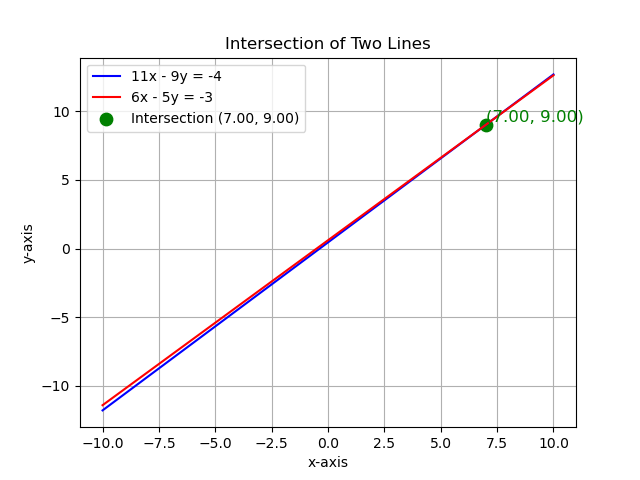
\includegraphics[width=0.75\textwidth]{figs/12.png}
    \caption{parallel lines}
    \label{fig:example_image}
\end{figure}
\end{frame}
\end{document}
